\documentclass{plantilla}
% --- Metadatos del Informe ---
\titulo{Trabajo práctico Nro 1}
\autores{Filsinger Gonzalo, Perea Ignacio, Parfait Manuel}
\materia{Electrónica Aplicada II}
\comision{4R2}

\begin{document}

\maketitle

\begin{abstract}
En este informe se abordará...
\end{abstract}

\begin{IEEEkeywords}
Ganancia, impedancia, desensibilidad, frecuencias.
\end{IEEEkeywords}

\section{Introducción}
\IEEEPARstart{E}{n} el siguiente informe...

\raggedbottom

\section{Desarrollo Experimental}

\subsection{Mediciones de Ganancias}
Primero armamos el circuito y dejamos el lazo abierto:

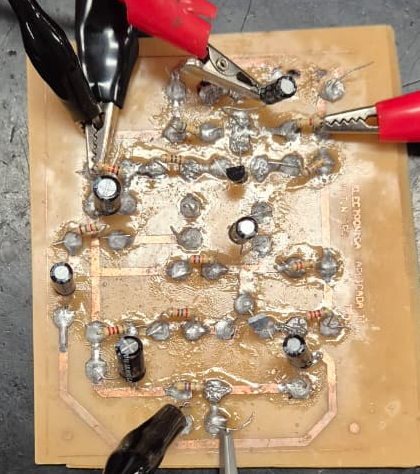
\includegraphics[width=0.35\textwidth]{images/circuito_lazoabierto.png}

Luego ponemos una señal de entrada con una amplitud arbitraria, en nuestro caso elegimos 130mVpp, y con el osciloscopio medimos la señal de salida.

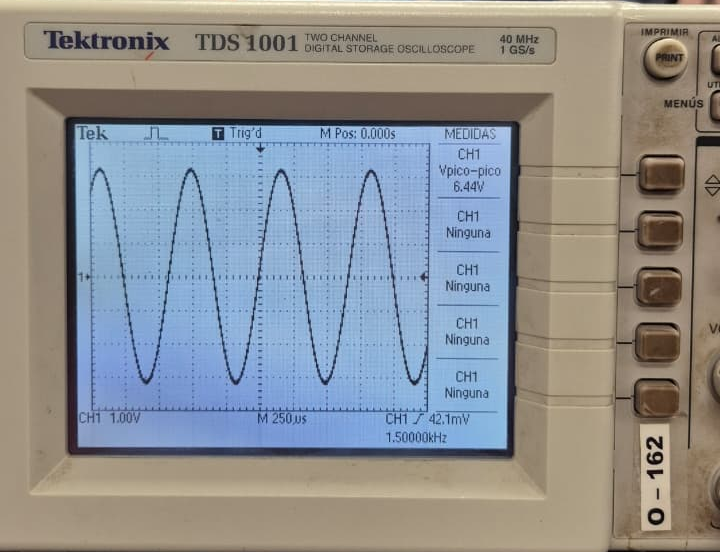
\includegraphics[width=0.35\textwidth]{images/osc_voabierto.png}

Podemos observar que para lazo abierto la señal de salida es de 6.44Vpp, por lo tanto la ganancia para lazo abierto es de:

\begin{equation}
A_{V} = \frac{V_{out}}{V_{in}} = \frac{6.44Vpp}{130mVpp} = 49.5
\end{equation}

Luego cerramos el lazo y repetimos el mismo procedimiento para medir la ganancia para lazo cerrado:


\begin{center}
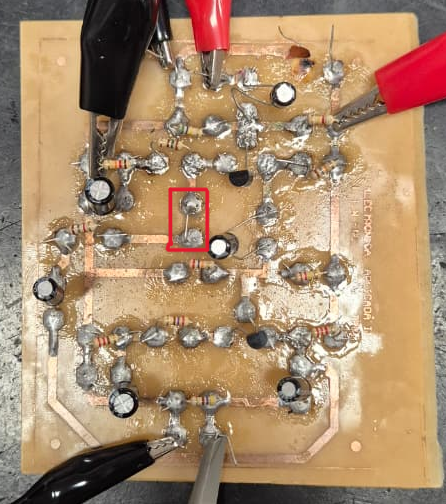
\includegraphics[width=0.35\textwidth]{images/circuito_lazocerrado.png}
\end{center}

\begin{figure}[H]
\centering
\begin{minipage}{0.35\textwidth}
\centering
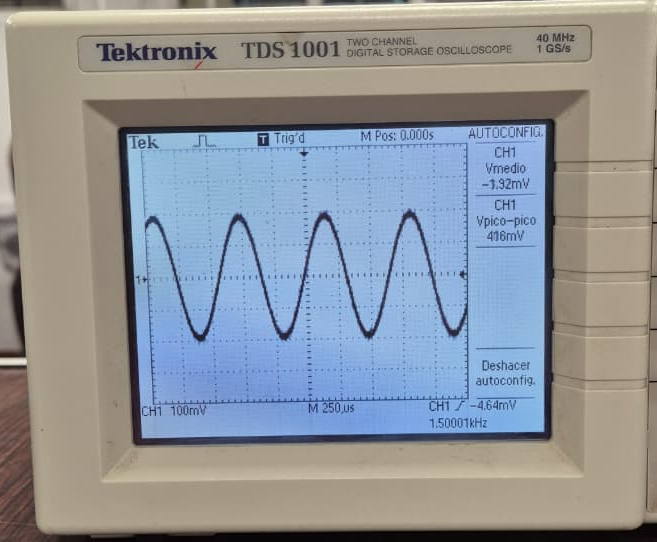
\includegraphics[width=\linewidth]{images/osc_vicerrado.png}
\end{minipage}\hfill
\begin{minipage}{0.35\textwidth}
\centering
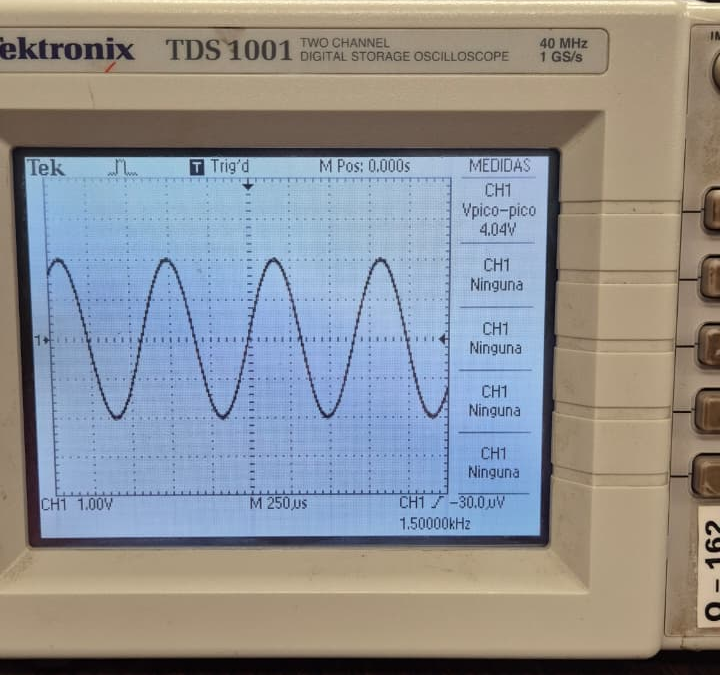
\includegraphics[width=\linewidth]{images/osc_vocerrado.png}
\end{minipage}
\end{figure}

Como podemos observar, ahora usamos un valor de 400mVpp para la entrada y la salida es de 4.04Vpp; por lo tanto, la ganancia para lazo cerrado es de:

\begin{equation}
A_{Vf} = \frac{V_{out}}{V_{in}} = \frac{4.04Vpp}{400mVpp} = 10.1
\end{equation}


Ahora para medir la desensibilidad, debemos modificar el circuito y reemplazar la resistencia emisora del segundo transistor por un trimpot multivuelta entre 500$\Omega$ y 1k$\Omega$. Hacemos variar el trimpot hasta que la ganancia de lazo abierto caiga en un 45\% respecto a su valor original, lo mismo para lazo cerrado, y con la siguiente fórmula calculamos la desensibilidad:

\begin{equation}
D = \frac{\Delta \% A_{V}}{\Delta \% A_{Vf}}
\end{equation}


\subsection{Mediciones de Impedancias}

Primero debemos llevar el circuito de lazo abierto a MES, para ello aumentaremos la señal de entrada hasta que esta se distorsione, y ajustaremos para llegar al punto máximo antes de la distorsión.
Como entrada tenemos 780mVpp.
\begin{center}
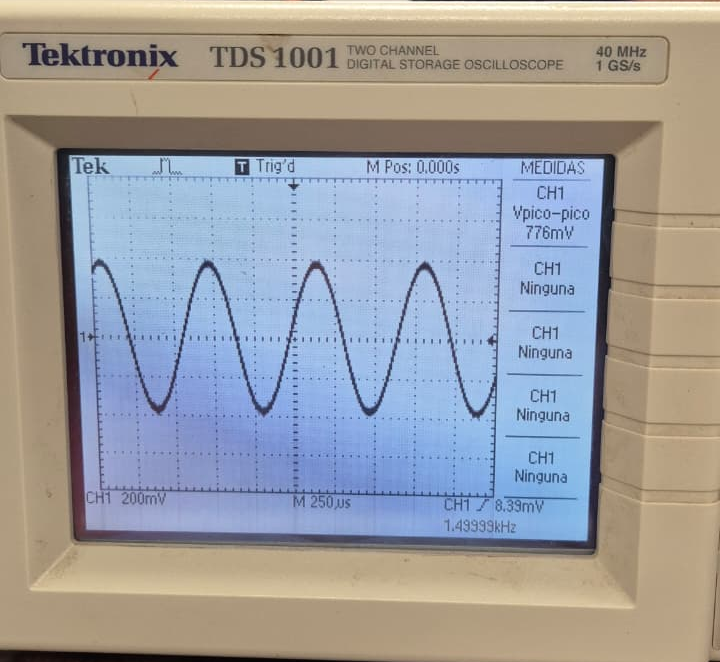
\includegraphics[width=0.35\textwidth]{images/osc_vimes.png}
\end{center}

Y como salida tenemos 46.8Vpp.


\begin{center}
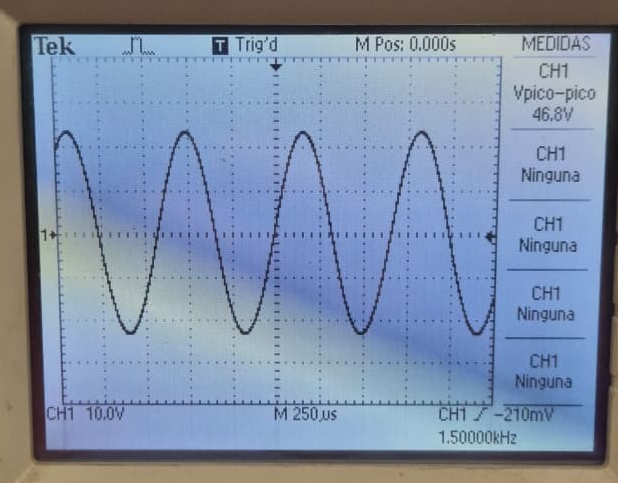
\includegraphics[width=0.35\textwidth]{images/osc_vomes.png}
\end{center}


Ahora colocamos un trimpot en la entrada del circuito para medir la impedancia de entrada, la forma de hacerlo es variar la resistencia del trimpot hasta que la señal de salida se reduzca a la mitad,es decir a 24.4Vpp, luego sacaremos el trimpot y mediremos su resistencia, esa será la impedancia de entrada del circuito.

\begin{center}
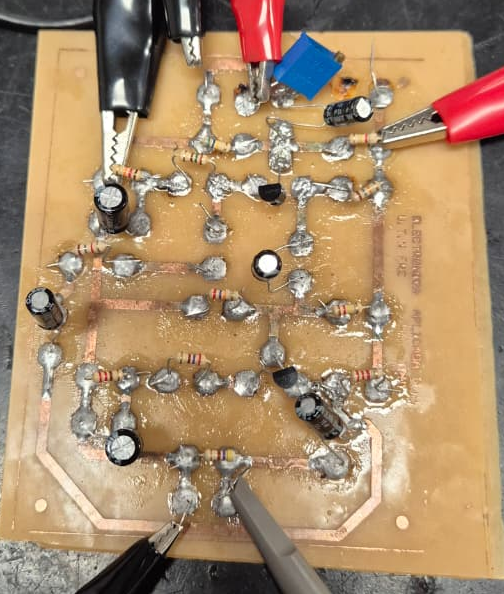
\includegraphics[width=0.35\textwidth]{images/circuito_impedanciaentrada.png}
\end{center}

\begin{center}
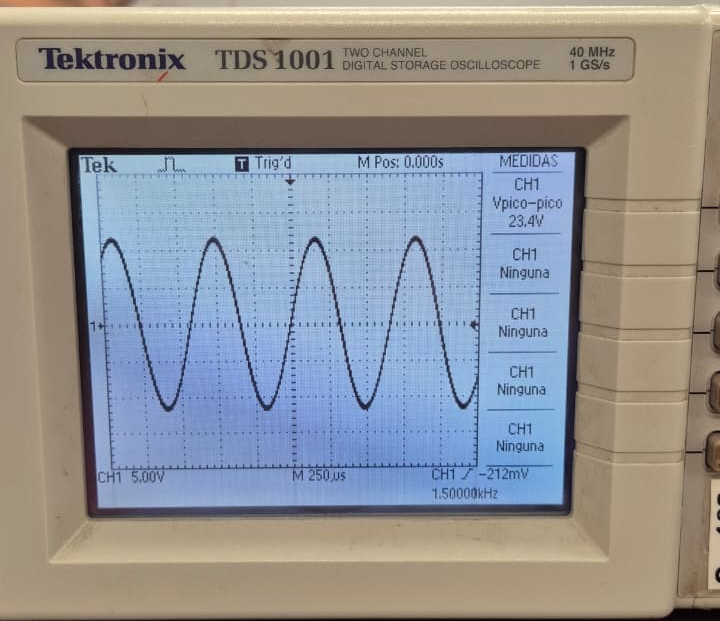
\includegraphics[width=0.35\textwidth]{images/osc_zi.png}
\end{center}

Al desconectar el trimpot y medir su resistencia, obtenemos un valor de XXXX, por lo tanto la impedancia de entrada del circuito es de XXXXX.

Luego para medir la impedancia de salida, colocamos el trimpot en la salida del circuito y repetimos el mismo procedimiento, variamos la resistencia del trimpot hasta que la señal de salida se reduzca a la mitad, luego sacamos el trimpot y medimos su resistencia, esa será la impedancia de salida del circuito.

Para podes calcular las impedancias de entrada y salida para lazo cerrado, utilizamos la desensibilidad calculada anteriormente y aplicamos las siguientes fórmulas:

\begin{equation}
Z_{if} = Z_{i} \cdot D
\end{equation}

\begin{equation}
Z_{of} = \frac{Z_{o}}{D}
\end{equation}


\subsection{Respuesta en Frecuencia}

Para medir la respuesta en frecuencia del circuito, utilizamos una señal de entrada con una amplitud constante y variamos la frecuencia de la señal de entrada, desde 10Hz hasta 2MHz, y medimos la señal de salida para cada frecuencia.

\begin{table}[H]
\begin{center}
\resizebox{0.8\columnwidth}{!}{%
\begin{tabular}{|
>{\columncolor[HTML]{FFCCC9}}c |c|c|}
\hline
\cellcolor[HTML]{FFCE93}Frecuencia {[}Hz{]} & \cellcolor[HTML]{FFCE93}Av & \cellcolor[HTML]{FFCE93}Avf \\ \hline
10      &  &  \\ \hline
100     &  &  \\ \hline
200     &  &  \\ \hline
500     &  &  \\ \hline
800     &  &  \\ \hline
1000    &  &  \\ \hline
1500    &  &  \\ \hline
2000    &  &  \\ \hline
5000    &  &  \\ \hline
8000    &  &  \\ \hline
10000   &  &  \\ \hline
50000   &  &  \\ \hline
100000  &  &  \\ \hline
200000  &  &  \\ \hline
400000  &  &  \\ \hline
500000  &  &  \\ \hline
800000  &  &  \\ \hline
1000000 &  &  \\ \hline
1500000 &  &  \\ \hline
2000000 &  &  \\ \hline
\end{tabular}%
}
\end{center}
\end{table}

De dicha tabla podemos graficar la respuesta en frecuencia del circuito

\subsection{Resultados}






\input{parte2}

\section{Conclusión}
Se logró verificar que...

% Referencias bibliográficas
\begin{thebibliography}{1}
\bibitem{IEEEhowto:kopka}
Fuentes...
\end{thebibliography}




\end{document}